\section{Results}

\subsection{Evaluation Against Other Approaches}

\begin{figure}[h]
    \centering
    \includegraphics[width=0.5\linewidth]{analysis/artefact/variation_approach/reduction_query_execution_time}
    \caption{
        This figure compares the type index with the LDP approach against other approaches.
        The shape index approach is better or similar to the other approaches except with S4.
    }
    \label{fig:compApproach}
\end{figure}


Figure~\ref{fig:compApproach} shows that the shape index approach for all query templates except S4 performs better or comparably to the Solid Pod network optimal traversal algorithm.
Queries can require as little as 13\% (S1) of the execution time of the Solid Pod network optimal traversal algorithm.
Queries that perform best are those where the number of HTTP requests decreased the most.
Table~\ref{tab:statSignificanceStateOfTheArt} in the \nameref{sec:appendix} presents an analysis of the statistical significance of the query template and its relation to the ratio of HTTP requests performed.
Query templates D6 and D7 show no reduction because they require nearly every document in the dataset to be processed by the engine, making our approach ineffective in these cases.
We notice that query template S4 with the shape index performed worse in every instance, with an increase in query execution time of up to 2.80 times.
This is further illustrated in Table~\ref{tab:ratioUsefulResources}, which shows that for these queries, the Solid Pod network optimal traversal algorithm achieves a ratio of useful resources dereferenced of 100\% or 50\%, compared to only 6\% with the shape index approach.
The poor performance is due to the fact that other approaches rely solely on the reachability \texttt{Cmatch}~\cite{hartig2016walking} to achieve completeness, without leveraging the structural properties of the datasets.
In contrast, the shape index approach always enforces the use of these properties, resulting in additional HTTP requests and increased processing time.
It has to be highlighted that our formalization assumes that structural assumptions are always used and that the shape index, if present, will be part of the traversal, see section~\ref{sec:sourceSelection}.
However, those queries were already fast, with the Solid Pod network optimal traversal algorithm approach being executed in approximately 0.30\% of the maximum execution time allowed.
Nonetheless, these results still highlight a category of queries and networks for which our approach is not well-suited.

The empirical evaluation of the query-containment algorithm shows that its execution time with the more detailed shapes from our experiment is negligible, with a maximum execution time of 4.655 ms (0.0039\% of the timeout).
The result tables are available in the supplementary material.
This outcome is expected, as the algorithm has polynomial time complexity, and the shapes and queries in the experiments are small and not deeply nested.
This suggests that the primary overhead in this approach is not from the algorithm itself but likely from the state retention required for the pruning reachability criteria.

\begin{figure}[htbp]
    \centering
    % First figure
    \begin{minipage}[t]{0.45\linewidth}
        \centering
        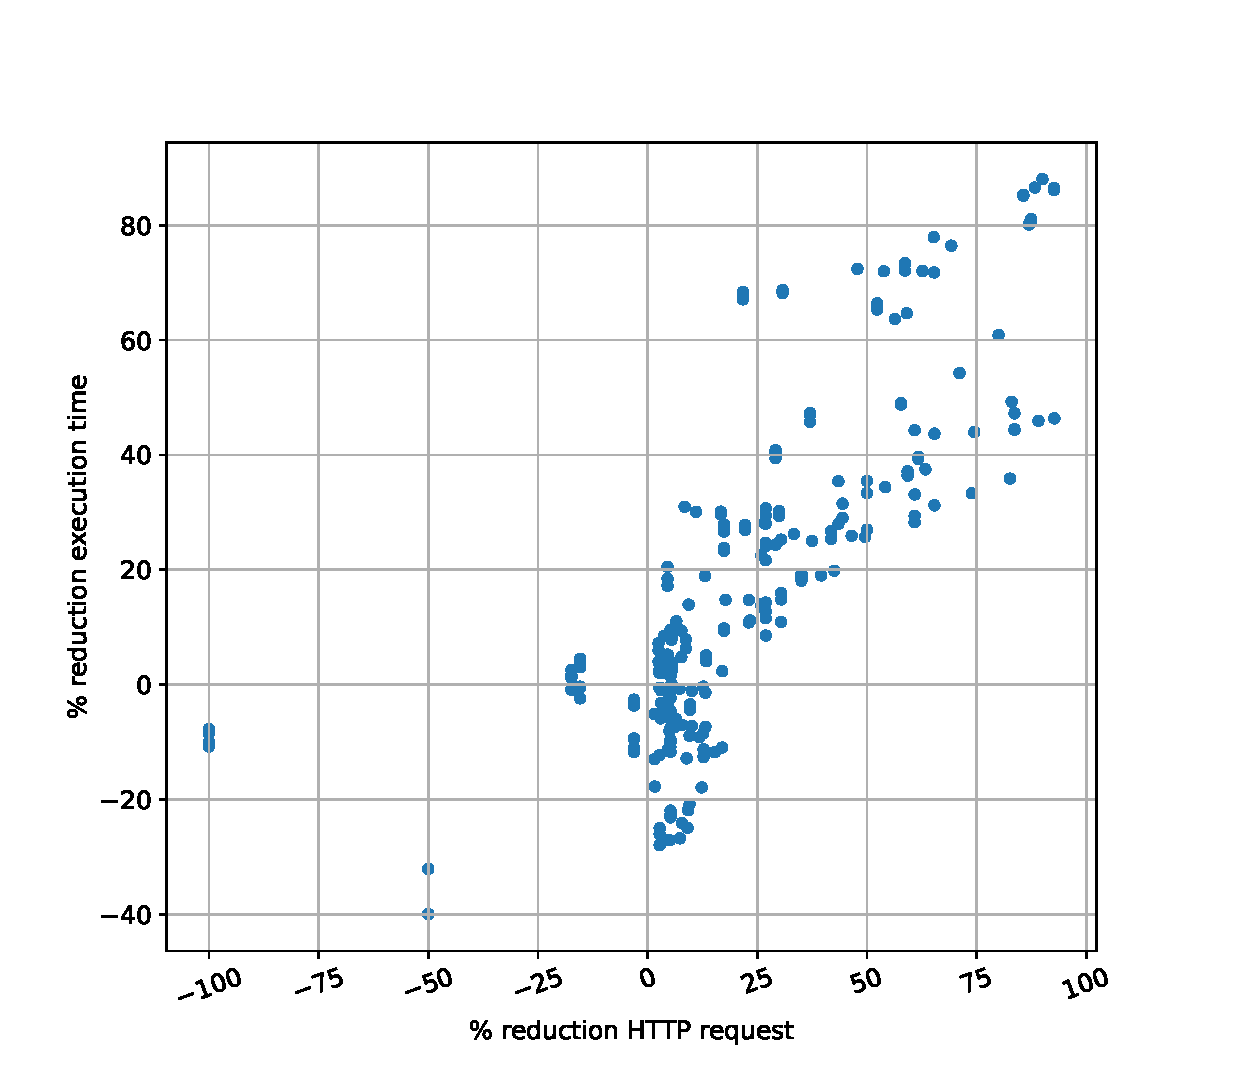
\includegraphics[width=\linewidth]{analysis/artefact/http_req_exec_time_relation/http_req_exec_time_cor_better}
        \label{fig:http_req_exec_time_cor_better}
    \end{minipage}
    \hspace{0.05\textwidth}
    % Second figure
    \begin{minipage}[t]{0.45\linewidth}
        \centering
        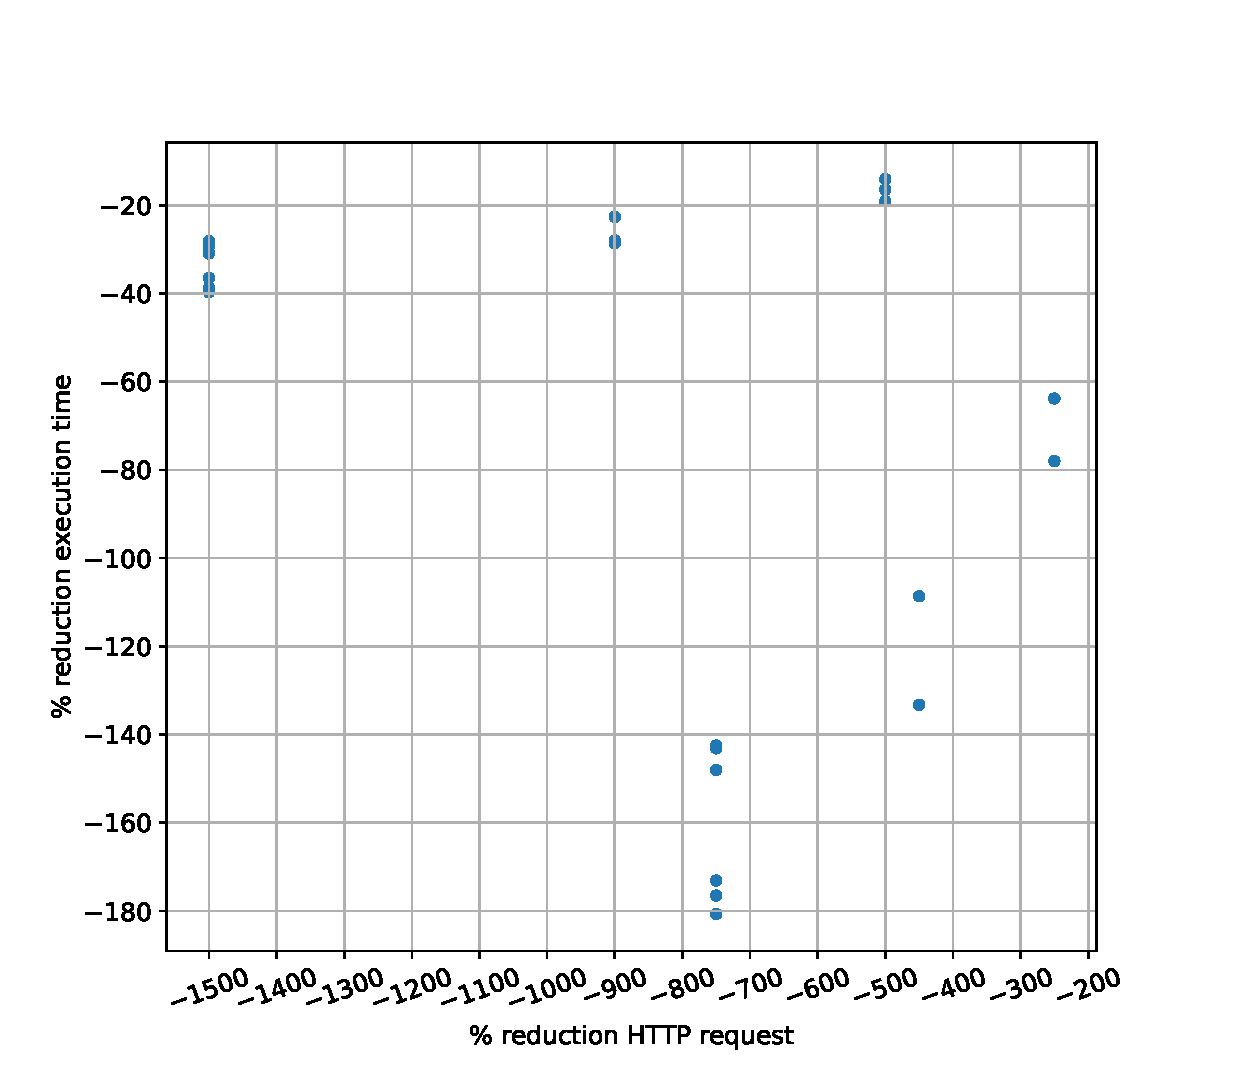
\includegraphics[width=\linewidth]{analysis/artefact/http_req_exec_time_relation/http_req_exec_time_cor_worse}
        \label{fig:http_req_exec_time_cor_worse}
    \end{minipage}

    % General caption
    \caption{
        The data show two regimes in the relation between the number of HTTP requests and the execution time, 
        we see a more linear correlation on the left figure than on the right figure.
        }
    \label{fig:http_req_exec_time_cor}
\end{figure}

To determine the relationship between the reduction of HTTP requests and the query execution time, we evaluated their ratio using 
the data of our experiments with the Solid Pod network optimal traversal algorithm results as the baseline.
We use Figure~\ref{fig:http_req_exec_time_cor} as a tool of analysis.
The relationship between HTTP request and query execution time can be divided into two regimes.
In the first regime (left figure), where the shape index approach reduces the number of HTTP requests, we notice a positive linear correlation with a
Pearson correlation coefficient (PCC) of 0.84 and a high statistical significance given a p-value of 3.00E-93.
However, evaluating an $R^2$ score with an exponential best fit curve we get a score of 0.72 and 0.71 for a linear curve.
We can notice that toward the end, the curve appears to exhibit more exponential behavior.
Below a ratio of approximately 0.83 of HTTP requests, the shape index approach did not guarantee a reduction in query execution time.
With this obsevation, the exponential behavior might be explained by the approach's overhead. 
It is possible that with a small reduction of HTTP requests, the state retention required for the pruning reachability criteria could offset the gain in the reduction of HTTP requests.
In the second regime (right figure), the shape index increases the number of HTTP requests.
We notice a weaker positive linear correlation with a PCC of 0.44 and a high statistical significance given a p-value of 9.01E-05 though the significance is lower than in the first regime.
The overall correlation between reducing HTTP requests and query execution time is positively linear, with a PCC of 0.56 and a high statistical significance with a p-value of 5.83E-36.
The overall correlation is more linear than exponential with $R^2$ scores respectively of 0.31 and 0.24, however due to the low score it is difficult to determine the nature of the distribution.
Explaining the two regimes' behavior exhibited by the data is challenging.
A possible explanation can be the lack of samples when the shape index approach performs poorly.
However, we can also notice that the relationship between the two variables in the first regime is closer to one-on-one (slope of approximately 0.91) than in the second regime (slope of approximately 0.08), where the ratio of HTTP requests has less of an impact.
This observation can lead us to question how complex the queries are in that regime; we can notice that the queries where the shape index increases vastly in the number 
of HTTP requests are the queries from the S4 template. 
However, those queries were already answered quickly and consisted of only four triple patterns and a union statement (with the alternative property path). 
Thus, it is possible that the number of HTTP requests has less of an impact because it is easier for the engine to perform the join operation upon reception of the data than when processing more complex queries.
% Analysis by query template? But we lack the space. In the appendix too...
% We can also with that explain some big gap in the plot.


\begin{figure}[h]
    \centering
    \includegraphics[width=0.95\linewidth]{analysis/artefact/variation_shape_index_all/plot}
    \caption{
    Shape index approaches tend to perform less effectively with limited network information and comparatively better where the baseline shape index underperforms.
    However, the utility of shape index information can vary depending on the specific queries and network characteristics.
    }
    \label{fig:adaptShapeIndex}
\end{figure}

\subsection{Evaluation of the Adaptivity}

The final part of the results analysis focuses on the adaptivity of the shape index approach.
In this analysis, we examine the impact of reducing the shape index information in the network and compare the results with a network in which all pods are exposed to detailed, complete shape indexes.
Figure~\ref{fig:adaptShapeIndex} presents three plots that illustrate the results of our evaluation of the approach's adaptivity.
The plot on the left shows the variation in the percentage of shape index across the network. 
As expected, we observe that queries that performed better in Figure~\ref{fig:compApproach} tend to perform worse with reduced shape index information, while queries that performed poorly improve. 
Queries that were unaffected by the shape index changes remain unaffected.
The plot in the middle shows the variation in the percentage of shape index entries using closed shapes.
The results here are more nuanced.
While there is a general trend for query evaluations with a lower percentage of closed shapes to behave similarly to the plot on the left, we also observe both performance gains and a drastic performance loss for query S1 when 80\% of the shape entries are closed.
The performance gain occurs because not every entry needs to be closed to affect query performance.
Entries mapped to an open shape are always considered relevant.
If the containment resolution leads to the same conclusion then if the entry is closed the execution will be more expensive. 
Additionally, shapes can be nested, and when open shapes are used, we do not need to dereference the nested shapes.
For query S1, with 80\% of closed shape entries, the performance lost was due to random chance, as the discriminatory entries were provided with open shapes in multiple instances when looking at the raw data.
The right plot shows the variation in the level of detail of the shapes.
Most queries tend to perform similarly or better, with the exception of S1.
Upon analyzing the output of our query containment algorithm, we observe that the additional information provided in our base approach does not affect the algorithm’s results.
However, the engine needs to dereference more shapes, which can decrease the execution time.
Query S1 is the only one where the added information can discriminate multiple parts of the datasets' domain, indicating the intuitive results that, in some situations, adding more information can be beneficial.
This sensitivity to the quality of the information in the index also helps explain the results for S1 in the middle plot. 
In that case, the query engine still had to dereference sources from each dataset, and the information available was likely insufficient to significantly discriminate between sources.

\subsection{Evaluation of Hypotheses}
In this section, we revisit our hypotheses.
\textbf{H1} is mostly valid as the shape index reduces HTTP requests for queries using structural properties, though it can drastically increase requests when such properties are not used.
\textbf{H2} is valid when HTTP requests are reduced, but near a ratio of 0.83, further reduction has diminishing impact due to exponential behavior.
However, its validity is questionable when considering the increase in the number of HTTP requests.
\textbf{H3} is valid, with the algorithm operating in polynomial time and completing under 4.655 ms in our benchmark.
\textbf{H4} is mainly invalid; reducing information rarely affected or benefited queries, except one case where it negated the performance gain from the shape index.
Thus, this outcome is query-dependent.
\textbf{H5} and \textbf{H6} are valid but show that the completeness of shape indexes has less impact on performance than their presence.
Queries benefiting most from the index were more affected, and gains were also seen in some negatively impacted queries.
Like \textbf{H4}, these findings are query-dependent.

